\documentclass[tikz,border=2pt]{standalone}
\usepackage{amsmath,amssymb}
\usepackage{pgfplots}
\pgfplotsset{compat=1.18}
\usetikzlibrary{arrows.meta}
\begin{document}
% Poisson in GLM form: b(theta) = e^theta. At theta = log 2 (lambda = 2) the tangent slope is
% b'(theta) = mu = 2 and the curvature b''(theta) = Var(Y) = 2 (a(phi) = 1).
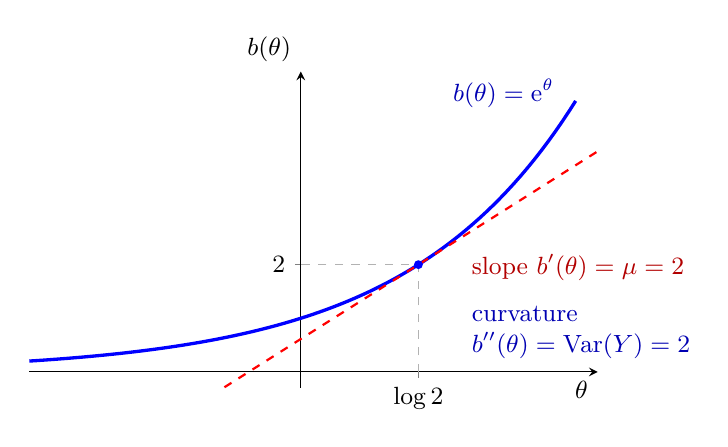
\begin{tikzpicture}[font=\small, >={Latex[length=2mm]}]
  \begin{axis}[
    axis lines=middle, xmin=-1.6, xmax=1.75, ymin=-0.3, ymax=5.6,
    xtick={0.6931}, xticklabels={$\log 2$}, ytick={2},
    xlabel={$\theta$}, ylabel={$b(\theta)$},
    xlabel style={anchor=north east}, ylabel style={anchor=south east},
    width=8.8cm, height=5.6cm, clip=false
    ]
    \addplot[blue, very thick, domain=-1.6:1.62, samples=80] {exp(x)};
    \addplot[red, thick, dashed, domain=-0.45:1.75, samples=2] {2+2*(x-0.6931)};
    \draw[gray!60, thin, dashed] (axis cs:0.6931,0) -- (axis cs:0.6931,2) -- (axis cs:0,2);
    \fill[blue] (axis cs:0.6931,2) circle (1.6pt);
    \node[blue!70!black, anchor=south east] at (axis cs:1.55,4.75) {$b(\theta)=\mathrm{e}^{\theta}$};
    \node[red!70!black, anchor=west] at (axis cs:0.95,1.95) {slope $b'(\theta)=\mu=2$};
    \node[blue!70!black, anchor=north west, align=left] at (axis cs:0.95,1.4) {curvature\\$b''(\theta)=\operatorname{Var}(Y)=2$};
  \end{axis}
\end{tikzpicture}
\end{document}
